% Created by tikzDevice version 0.6.2-92-0ad2792 on 2013-03-06 11:29:20
% !TEX encoding = UTF-8 Unicode
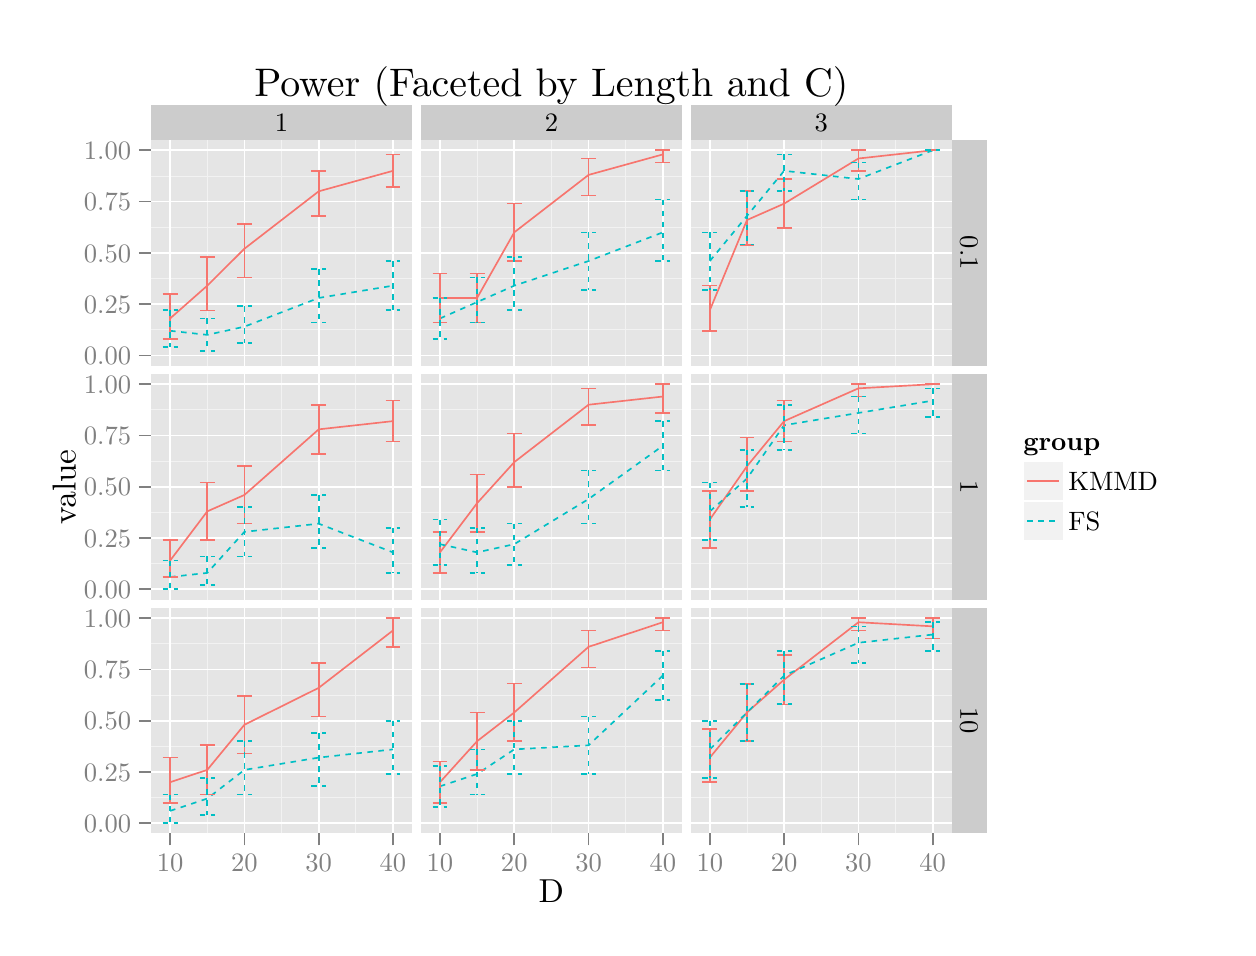
\begin{tikzpicture}[x=1pt,y=1pt]
\definecolor[named]{fillColor}{rgb}{1.00,1.00,1.00}
\path[use as bounding box,fill=fillColor,fill opacity=0.00] (0,0) rectangle (433.62,325.21);
\begin{scope}
\path[clip] (  0.00,  0.00) rectangle (433.62,325.21);
\definecolor[named]{drawColor}{rgb}{1.00,1.00,1.00}
\definecolor[named]{fillColor}{rgb}{1.00,1.00,1.00}

\path[draw=drawColor,line width= 0.6pt,line join=round,line cap=round,fill=fillColor] (  0.00,  0.00) rectangle (433.62,325.21);
\end{scope}
\begin{scope}
\path[clip] ( 44.49,284.60) rectangle (138.99,297.23);
\definecolor[named]{fillColor}{rgb}{0.80,0.80,0.80}

\path[fill=fillColor] ( 44.49,284.60) rectangle (138.99,297.23);
\definecolor[named]{drawColor}{rgb}{0.00,0.00,0.00}

\node[text=drawColor,anchor=base,inner sep=0pt, outer sep=0pt, scale=  0.96] at ( 91.74,287.61) {1};
\end{scope}
\begin{scope}
\path[clip] (142.00,284.60) rectangle (236.50,297.23);
\definecolor[named]{fillColor}{rgb}{0.80,0.80,0.80}

\path[fill=fillColor] (142.00,284.60) rectangle (236.50,297.23);
\definecolor[named]{drawColor}{rgb}{0.00,0.00,0.00}

\node[text=drawColor,anchor=base,inner sep=0pt, outer sep=0pt, scale=  0.96] at (189.25,287.61) {2};
\end{scope}
\begin{scope}
\path[clip] (239.51,284.60) rectangle (334.02,297.23);
\definecolor[named]{fillColor}{rgb}{0.80,0.80,0.80}

\path[fill=fillColor] (239.51,284.60) rectangle (334.02,297.23);
\definecolor[named]{drawColor}{rgb}{0.00,0.00,0.00}

\node[text=drawColor,anchor=base,inner sep=0pt, outer sep=0pt, scale=  0.96] at (286.76,287.61) {3};
\end{scope}
\begin{scope}
\path[clip] ( 44.49,203.08) rectangle (138.99,284.60);
\definecolor[named]{fillColor}{rgb}{0.90,0.90,0.90}

\path[fill=fillColor] ( 44.49,203.08) rectangle (138.99,284.60);
\definecolor[named]{drawColor}{rgb}{0.95,0.95,0.95}

\path[draw=drawColor,line width= 0.3pt,line join=round] ( 44.49,216.05) --
	(138.99,216.05);

\path[draw=drawColor,line width= 0.3pt,line join=round] ( 44.49,234.58) --
	(138.99,234.58);

\path[draw=drawColor,line width= 0.3pt,line join=round] ( 44.49,253.10) --
	(138.99,253.10);

\path[draw=drawColor,line width= 0.3pt,line join=round] ( 44.49,271.63) --
	(138.99,271.63);

\path[draw=drawColor,line width= 0.3pt,line join=round] ( 64.89,203.08) --
	( 64.89,284.60);

\path[draw=drawColor,line width= 0.3pt,line join=round] ( 91.74,203.08) --
	( 91.74,284.60);

\path[draw=drawColor,line width= 0.3pt,line join=round] (118.58,203.08) --
	(118.58,284.60);
\definecolor[named]{drawColor}{rgb}{1.00,1.00,1.00}

\path[draw=drawColor,line width= 0.6pt,line join=round] ( 44.49,206.79) --
	(138.99,206.79);

\path[draw=drawColor,line width= 0.6pt,line join=round] ( 44.49,225.31) --
	(138.99,225.31);

\path[draw=drawColor,line width= 0.6pt,line join=round] ( 44.49,243.84) --
	(138.99,243.84);

\path[draw=drawColor,line width= 0.6pt,line join=round] ( 44.49,262.36) --
	(138.99,262.36);

\path[draw=drawColor,line width= 0.6pt,line join=round] ( 44.49,280.89) --
	(138.99,280.89);

\path[draw=drawColor,line width= 0.6pt,line join=round] ( 51.47,203.08) --
	( 51.47,284.60);

\path[draw=drawColor,line width= 0.6pt,line join=round] ( 78.31,203.08) --
	( 78.31,284.60);

\path[draw=drawColor,line width= 0.6pt,line join=round] (105.16,203.08) --
	(105.16,284.60);

\path[draw=drawColor,line width= 0.6pt,line join=round] (132.01,203.08) --
	(132.01,284.60);
\definecolor[named]{drawColor}{rgb}{0.97,0.46,0.43}

\path[draw=drawColor,line width= 0.6pt,line join=round] ( 51.47,220.13) --
	( 64.89,231.98) --
	( 78.31,245.32) --
	(105.16,266.07) --
	(132.01,273.48);
\definecolor[named]{drawColor}{rgb}{0.00,0.75,0.77}

\path[draw=drawColor,line width= 0.6pt,dash pattern=on 2pt off 2pt ,line join=round] ( 51.47,215.68) --
	( 64.89,214.20) --
	( 78.31,217.16) --
	(105.16,227.54) --
	(132.01,231.98);
\definecolor[named]{drawColor}{rgb}{0.97,0.46,0.43}

\path[draw=drawColor,line width= 0.6pt,line join=round] ( 48.78,229.02) --
	( 54.15,229.02);

\path[draw=drawColor,line width= 0.6pt,line join=round] ( 51.47,229.02) --
	( 51.47,212.72);

\path[draw=drawColor,line width= 0.6pt,line join=round] ( 48.78,212.72) --
	( 54.15,212.72);

\path[draw=drawColor,line width= 0.6pt,line join=round] ( 62.20,242.36) --
	( 67.57,242.36);

\path[draw=drawColor,line width= 0.6pt,line join=round] ( 64.89,242.36) --
	( 64.89,223.05);

\path[draw=drawColor,line width= 0.6pt,line join=round] ( 62.20,223.05) --
	( 67.57,223.05);

\path[draw=drawColor,line width= 0.6pt,line join=round] ( 75.63,254.25) --
	( 81.00,254.25);

\path[draw=drawColor,line width= 0.6pt,line join=round] ( 78.31,254.25) --
	( 78.31,234.95);

\path[draw=drawColor,line width= 0.6pt,line join=round] ( 75.63,234.95) --
	( 81.00,234.95);

\path[draw=drawColor,line width= 0.6pt,line join=round] (102.48,273.48) --
	(107.85,273.48);

\path[draw=drawColor,line width= 0.6pt,line join=round] (105.16,273.48) --
	(105.16,257.18);

\path[draw=drawColor,line width= 0.6pt,line join=round] (102.48,257.18) --
	(107.85,257.18);

\path[draw=drawColor,line width= 0.6pt,line join=round] (129.32,279.41) --
	(134.69,279.41);

\path[draw=drawColor,line width= 0.6pt,line join=round] (132.01,279.41) --
	(132.01,267.55);

\path[draw=drawColor,line width= 0.6pt,line join=round] (129.32,267.55) --
	(134.69,267.55);
\definecolor[named]{drawColor}{rgb}{0.00,0.75,0.77}

\path[draw=drawColor,line width= 0.6pt,dash pattern=on 2pt off 2pt ,line join=round] ( 48.78,223.09) --
	( 54.15,223.09);

\path[draw=drawColor,line width= 0.6pt,dash pattern=on 2pt off 2pt ,line join=round] ( 51.47,223.09) --
	( 51.47,209.75);

\path[draw=drawColor,line width= 0.6pt,dash pattern=on 2pt off 2pt ,line join=round] ( 48.78,209.75) --
	( 54.15,209.75);

\path[draw=drawColor,line width= 0.6pt,dash pattern=on 2pt off 2pt ,line join=round] ( 62.20,220.13) --
	( 67.57,220.13);

\path[draw=drawColor,line width= 0.6pt,dash pattern=on 2pt off 2pt ,line join=round] ( 64.89,220.13) --
	( 64.89,208.27);

\path[draw=drawColor,line width= 0.6pt,dash pattern=on 2pt off 2pt ,line join=round] ( 62.20,208.27) --
	( 67.57,208.27);

\path[draw=drawColor,line width= 0.6pt,dash pattern=on 2pt off 2pt ,line join=round] ( 75.63,224.57) --
	( 81.00,224.57);

\path[draw=drawColor,line width= 0.6pt,dash pattern=on 2pt off 2pt ,line join=round] ( 78.31,224.57) --
	( 78.31,211.23);

\path[draw=drawColor,line width= 0.6pt,dash pattern=on 2pt off 2pt ,line join=round] ( 75.63,211.23) --
	( 81.00,211.23);

\path[draw=drawColor,line width= 0.6pt,dash pattern=on 2pt off 2pt ,line join=round] (102.48,237.91) --
	(107.85,237.91);

\path[draw=drawColor,line width= 0.6pt,dash pattern=on 2pt off 2pt ,line join=round] (105.16,237.91) --
	(105.16,218.64);

\path[draw=drawColor,line width= 0.6pt,dash pattern=on 2pt off 2pt ,line join=round] (102.48,218.64) --
	(107.85,218.64);

\path[draw=drawColor,line width= 0.6pt,dash pattern=on 2pt off 2pt ,line join=round] (129.32,240.88) --
	(134.69,240.88);

\path[draw=drawColor,line width= 0.6pt,dash pattern=on 2pt off 2pt ,line join=round] (132.01,240.88) --
	(132.01,223.09);

\path[draw=drawColor,line width= 0.6pt,dash pattern=on 2pt off 2pt ,line join=round] (129.32,223.09) --
	(134.69,223.09);
\end{scope}
\begin{scope}
\path[clip] ( 44.49,118.56) rectangle (138.99,200.07);
\definecolor[named]{fillColor}{rgb}{0.90,0.90,0.90}

\path[fill=fillColor] ( 44.49,118.56) rectangle (138.99,200.07);
\definecolor[named]{drawColor}{rgb}{0.95,0.95,0.95}

\path[draw=drawColor,line width= 0.3pt,line join=round] ( 44.49,131.53) --
	(138.99,131.53);

\path[draw=drawColor,line width= 0.3pt,line join=round] ( 44.49,150.05) --
	(138.99,150.05);

\path[draw=drawColor,line width= 0.3pt,line join=round] ( 44.49,168.58) --
	(138.99,168.58);

\path[draw=drawColor,line width= 0.3pt,line join=round] ( 44.49,187.10) --
	(138.99,187.10);

\path[draw=drawColor,line width= 0.3pt,line join=round] ( 64.89,118.56) --
	( 64.89,200.07);

\path[draw=drawColor,line width= 0.3pt,line join=round] ( 91.74,118.56) --
	( 91.74,200.07);

\path[draw=drawColor,line width= 0.3pt,line join=round] (118.58,118.56) --
	(118.58,200.07);
\definecolor[named]{drawColor}{rgb}{1.00,1.00,1.00}

\path[draw=drawColor,line width= 0.6pt,line join=round] ( 44.49,122.26) --
	(138.99,122.26);

\path[draw=drawColor,line width= 0.6pt,line join=round] ( 44.49,140.79) --
	(138.99,140.79);

\path[draw=drawColor,line width= 0.6pt,line join=round] ( 44.49,159.32) --
	(138.99,159.32);

\path[draw=drawColor,line width= 0.6pt,line join=round] ( 44.49,177.84) --
	(138.99,177.84);

\path[draw=drawColor,line width= 0.6pt,line join=round] ( 44.49,196.37) --
	(138.99,196.37);

\path[draw=drawColor,line width= 0.6pt,line join=round] ( 51.47,118.56) --
	( 51.47,200.07);

\path[draw=drawColor,line width= 0.6pt,line join=round] ( 78.31,118.56) --
	( 78.31,200.07);

\path[draw=drawColor,line width= 0.6pt,line join=round] (105.16,118.56) --
	(105.16,200.07);

\path[draw=drawColor,line width= 0.6pt,line join=round] (132.01,118.56) --
	(132.01,200.07);
\definecolor[named]{drawColor}{rgb}{0.97,0.46,0.43}

\path[draw=drawColor,line width= 0.6pt,line join=round] ( 51.47,132.64) --
	( 64.89,150.42) --
	( 78.31,156.35) --
	(105.16,180.06) --
	(132.01,183.03);
\definecolor[named]{drawColor}{rgb}{0.00,0.75,0.77}

\path[draw=drawColor,line width= 0.6pt,dash pattern=on 2pt off 2pt ,line join=round] ( 51.47,126.71) --
	( 64.89,128.19) --
	( 78.31,143.01) --
	(105.16,145.98) --
	(132.01,135.60);
\definecolor[named]{drawColor}{rgb}{0.97,0.46,0.43}

\path[draw=drawColor,line width= 0.6pt,line join=round] ( 48.78,140.05) --
	( 54.15,140.05);

\path[draw=drawColor,line width= 0.6pt,line join=round] ( 51.47,140.05) --
	( 51.47,126.71);

\path[draw=drawColor,line width= 0.6pt,line join=round] ( 48.78,126.71) --
	( 54.15,126.71);

\path[draw=drawColor,line width= 0.6pt,line join=round] ( 62.20,160.80) --
	( 67.57,160.80);

\path[draw=drawColor,line width= 0.6pt,line join=round] ( 64.89,160.80) --
	( 64.89,140.05);

\path[draw=drawColor,line width= 0.6pt,line join=round] ( 62.20,140.05) --
	( 67.57,140.05);

\path[draw=drawColor,line width= 0.6pt,line join=round] ( 75.63,166.73) --
	( 81.00,166.73);

\path[draw=drawColor,line width= 0.6pt,line join=round] ( 78.31,166.73) --
	( 78.31,145.98);

\path[draw=drawColor,line width= 0.6pt,line join=round] ( 75.63,145.98) --
	( 81.00,145.98);

\path[draw=drawColor,line width= 0.6pt,line join=round] (102.48,188.96) --
	(107.85,188.96);

\path[draw=drawColor,line width= 0.6pt,line join=round] (105.16,188.96) --
	(105.16,171.17);

\path[draw=drawColor,line width= 0.6pt,line join=round] (102.48,171.17) --
	(107.85,171.17);

\path[draw=drawColor,line width= 0.6pt,line join=round] (129.32,190.44) --
	(134.69,190.44);

\path[draw=drawColor,line width= 0.6pt,line join=round] (132.01,190.44) --
	(132.01,175.62);

\path[draw=drawColor,line width= 0.6pt,line join=round] (129.32,175.62) --
	(134.69,175.62);
\definecolor[named]{drawColor}{rgb}{0.00,0.75,0.77}

\path[draw=drawColor,line width= 0.6pt,dash pattern=on 2pt off 2pt ,line join=round] ( 48.78,132.64) --
	( 54.15,132.64);

\path[draw=drawColor,line width= 0.6pt,dash pattern=on 2pt off 2pt ,line join=round] ( 51.47,132.64) --
	( 51.47,122.26);

\path[draw=drawColor,line width= 0.6pt,dash pattern=on 2pt off 2pt ,line join=round] ( 48.78,122.26) --
	( 54.15,122.26);

\path[draw=drawColor,line width= 0.6pt,dash pattern=on 2pt off 2pt ,line join=round] ( 62.20,134.12) --
	( 67.57,134.12);

\path[draw=drawColor,line width= 0.6pt,dash pattern=on 2pt off 2pt ,line join=round] ( 64.89,134.12) --
	( 64.89,123.75);

\path[draw=drawColor,line width= 0.6pt,dash pattern=on 2pt off 2pt ,line join=round] ( 62.20,123.75) --
	( 67.57,123.75);

\path[draw=drawColor,line width= 0.6pt,dash pattern=on 2pt off 2pt ,line join=round] ( 75.63,151.90) --
	( 81.00,151.90);

\path[draw=drawColor,line width= 0.6pt,dash pattern=on 2pt off 2pt ,line join=round] ( 78.31,151.90) --
	( 78.31,134.12);

\path[draw=drawColor,line width= 0.6pt,dash pattern=on 2pt off 2pt ,line join=round] ( 75.63,134.12) --
	( 81.00,134.12);

\path[draw=drawColor,line width= 0.6pt,dash pattern=on 2pt off 2pt ,line join=round] (102.48,156.35) --
	(107.85,156.35);

\path[draw=drawColor,line width= 0.6pt,dash pattern=on 2pt off 2pt ,line join=round] (105.16,156.35) --
	(105.16,137.08);

\path[draw=drawColor,line width= 0.6pt,dash pattern=on 2pt off 2pt ,line join=round] (102.48,137.08) --
	(107.85,137.08);

\path[draw=drawColor,line width= 0.6pt,dash pattern=on 2pt off 2pt ,line join=round] (129.32,144.49) --
	(134.69,144.49);

\path[draw=drawColor,line width= 0.6pt,dash pattern=on 2pt off 2pt ,line join=round] (132.01,144.49) --
	(132.01,128.19);

\path[draw=drawColor,line width= 0.6pt,dash pattern=on 2pt off 2pt ,line join=round] (129.32,128.19) --
	(134.69,128.19);
\end{scope}
\begin{scope}
\path[clip] ( 44.49, 34.03) rectangle (138.99,115.55);
\definecolor[named]{fillColor}{rgb}{0.90,0.90,0.90}

\path[fill=fillColor] ( 44.49, 34.03) rectangle (138.99,115.55);
\definecolor[named]{drawColor}{rgb}{0.95,0.95,0.95}

\path[draw=drawColor,line width= 0.3pt,line join=round] ( 44.49, 47.00) --
	(138.99, 47.00);

\path[draw=drawColor,line width= 0.3pt,line join=round] ( 44.49, 65.53) --
	(138.99, 65.53);

\path[draw=drawColor,line width= 0.3pt,line join=round] ( 44.49, 84.05) --
	(138.99, 84.05);

\path[draw=drawColor,line width= 0.3pt,line join=round] ( 44.49,102.58) --
	(138.99,102.58);

\path[draw=drawColor,line width= 0.3pt,line join=round] ( 64.89, 34.03) --
	( 64.89,115.55);

\path[draw=drawColor,line width= 0.3pt,line join=round] ( 91.74, 34.03) --
	( 91.74,115.55);

\path[draw=drawColor,line width= 0.3pt,line join=round] (118.58, 34.03) --
	(118.58,115.55);
\definecolor[named]{drawColor}{rgb}{1.00,1.00,1.00}

\path[draw=drawColor,line width= 0.6pt,line join=round] ( 44.49, 37.74) --
	(138.99, 37.74);

\path[draw=drawColor,line width= 0.6pt,line join=round] ( 44.49, 56.27) --
	(138.99, 56.27);

\path[draw=drawColor,line width= 0.6pt,line join=round] ( 44.49, 74.79) --
	(138.99, 74.79);

\path[draw=drawColor,line width= 0.6pt,line join=round] ( 44.49, 93.32) --
	(138.99, 93.32);

\path[draw=drawColor,line width= 0.6pt,line join=round] ( 44.49,111.84) --
	(138.99,111.84);

\path[draw=drawColor,line width= 0.6pt,line join=round] ( 51.47, 34.03) --
	( 51.47,115.55);

\path[draw=drawColor,line width= 0.6pt,line join=round] ( 78.31, 34.03) --
	( 78.31,115.55);

\path[draw=drawColor,line width= 0.6pt,line join=round] (105.16, 34.03) --
	(105.16,115.55);

\path[draw=drawColor,line width= 0.6pt,line join=round] (132.01, 34.03) --
	(132.01,115.55);
\definecolor[named]{drawColor}{rgb}{0.97,0.46,0.43}

\path[draw=drawColor,line width= 0.6pt,line join=round] ( 51.47, 52.56) --
	( 64.89, 57.01) --
	( 78.31, 73.31) --
	(105.16, 86.65) --
	(132.01,107.40);
\definecolor[named]{drawColor}{rgb}{0.00,0.75,0.77}

\path[draw=drawColor,line width= 0.6pt,dash pattern=on 2pt off 2pt ,line join=round] ( 51.47, 42.19) --
	( 64.89, 46.63) --
	( 78.31, 57.01) --
	(105.16, 61.45) --
	(132.01, 64.42);
\definecolor[named]{drawColor}{rgb}{0.97,0.46,0.43}

\path[draw=drawColor,line width= 0.6pt,line join=round] ( 48.78, 61.45) --
	( 54.15, 61.45);

\path[draw=drawColor,line width= 0.6pt,line join=round] ( 51.47, 61.45) --
	( 51.47, 45.15);

\path[draw=drawColor,line width= 0.6pt,line join=round] ( 48.78, 45.15) --
	( 54.15, 45.15);

\path[draw=drawColor,line width= 0.6pt,line join=round] ( 62.20, 65.90) --
	( 67.57, 65.90);

\path[draw=drawColor,line width= 0.6pt,line join=round] ( 64.89, 65.90) --
	( 64.89, 48.11);

\path[draw=drawColor,line width= 0.6pt,line join=round] ( 62.20, 48.11) --
	( 67.57, 48.11);

\path[draw=drawColor,line width= 0.6pt,line join=round] ( 75.63, 83.68) --
	( 81.00, 83.68);

\path[draw=drawColor,line width= 0.6pt,line join=round] ( 78.31, 83.68) --
	( 78.31, 62.93);

\path[draw=drawColor,line width= 0.6pt,line join=round] ( 75.63, 62.93) --
	( 81.00, 62.93);

\path[draw=drawColor,line width= 0.6pt,line join=round] (102.48, 95.54) --
	(107.85, 95.54);

\path[draw=drawColor,line width= 0.6pt,line join=round] (105.16, 95.54) --
	(105.16, 76.27);

\path[draw=drawColor,line width= 0.6pt,line join=round] (102.48, 76.27) --
	(107.85, 76.27);

\path[draw=drawColor,line width= 0.6pt,line join=round] (129.32,111.84) --
	(134.69,111.84);

\path[draw=drawColor,line width= 0.6pt,line join=round] (132.01,111.84) --
	(132.01,101.47);

\path[draw=drawColor,line width= 0.6pt,line join=round] (129.32,101.47) --
	(134.69,101.47);
\definecolor[named]{drawColor}{rgb}{0.00,0.75,0.77}

\path[draw=drawColor,line width= 0.6pt,dash pattern=on 2pt off 2pt ,line join=round] ( 48.78, 48.11) --
	( 54.15, 48.11);

\path[draw=drawColor,line width= 0.6pt,dash pattern=on 2pt off 2pt ,line join=round] ( 51.47, 48.11) --
	( 51.47, 37.74);

\path[draw=drawColor,line width= 0.6pt,dash pattern=on 2pt off 2pt ,line join=round] ( 48.78, 37.74) --
	( 54.15, 37.74);

\path[draw=drawColor,line width= 0.6pt,dash pattern=on 2pt off 2pt ,line join=round] ( 62.20, 54.04) --
	( 67.57, 54.04);

\path[draw=drawColor,line width= 0.6pt,dash pattern=on 2pt off 2pt ,line join=round] ( 64.89, 54.04) --
	( 64.89, 40.70);

\path[draw=drawColor,line width= 0.6pt,dash pattern=on 2pt off 2pt ,line join=round] ( 62.20, 40.70) --
	( 67.57, 40.70);

\path[draw=drawColor,line width= 0.6pt,dash pattern=on 2pt off 2pt ,line join=round] ( 75.63, 67.38) --
	( 81.00, 67.38);

\path[draw=drawColor,line width= 0.6pt,dash pattern=on 2pt off 2pt ,line join=round] ( 78.31, 67.38) --
	( 78.31, 48.11);

\path[draw=drawColor,line width= 0.6pt,dash pattern=on 2pt off 2pt ,line join=round] ( 75.63, 48.11) --
	( 81.00, 48.11);

\path[draw=drawColor,line width= 0.6pt,dash pattern=on 2pt off 2pt ,line join=round] (102.48, 70.34) --
	(107.85, 70.34);

\path[draw=drawColor,line width= 0.6pt,dash pattern=on 2pt off 2pt ,line join=round] (105.16, 70.34) --
	(105.16, 51.08);

\path[draw=drawColor,line width= 0.6pt,dash pattern=on 2pt off 2pt ,line join=round] (102.48, 51.08) --
	(107.85, 51.08);

\path[draw=drawColor,line width= 0.6pt,dash pattern=on 2pt off 2pt ,line join=round] (129.32, 74.79) --
	(134.69, 74.79);

\path[draw=drawColor,line width= 0.6pt,dash pattern=on 2pt off 2pt ,line join=round] (132.01, 74.79) --
	(132.01, 55.52);

\path[draw=drawColor,line width= 0.6pt,dash pattern=on 2pt off 2pt ,line join=round] (129.32, 55.52) --
	(134.69, 55.52);
\end{scope}
\begin{scope}
\path[clip] (142.00,203.08) rectangle (236.50,284.60);
\definecolor[named]{fillColor}{rgb}{0.90,0.90,0.90}

\path[fill=fillColor] (142.00,203.08) rectangle (236.50,284.60);
\definecolor[named]{drawColor}{rgb}{0.95,0.95,0.95}

\path[draw=drawColor,line width= 0.3pt,line join=round] (142.00,216.05) --
	(236.50,216.05);

\path[draw=drawColor,line width= 0.3pt,line join=round] (142.00,234.58) --
	(236.50,234.58);

\path[draw=drawColor,line width= 0.3pt,line join=round] (142.00,253.10) --
	(236.50,253.10);

\path[draw=drawColor,line width= 0.3pt,line join=round] (142.00,271.63) --
	(236.50,271.63);

\path[draw=drawColor,line width= 0.3pt,line join=round] (162.40,203.08) --
	(162.40,284.60);

\path[draw=drawColor,line width= 0.3pt,line join=round] (189.25,203.08) --
	(189.25,284.60);

\path[draw=drawColor,line width= 0.3pt,line join=round] (216.10,203.08) --
	(216.10,284.60);
\definecolor[named]{drawColor}{rgb}{1.00,1.00,1.00}

\path[draw=drawColor,line width= 0.6pt,line join=round] (142.00,206.79) --
	(236.50,206.79);

\path[draw=drawColor,line width= 0.6pt,line join=round] (142.00,225.31) --
	(236.50,225.31);

\path[draw=drawColor,line width= 0.6pt,line join=round] (142.00,243.84) --
	(236.50,243.84);

\path[draw=drawColor,line width= 0.6pt,line join=round] (142.00,262.36) --
	(236.50,262.36);

\path[draw=drawColor,line width= 0.6pt,line join=round] (142.00,280.89) --
	(236.50,280.89);

\path[draw=drawColor,line width= 0.6pt,line join=round] (148.98,203.08) --
	(148.98,284.60);

\path[draw=drawColor,line width= 0.6pt,line join=round] (175.83,203.08) --
	(175.83,284.60);

\path[draw=drawColor,line width= 0.6pt,line join=round] (202.67,203.08) --
	(202.67,284.60);

\path[draw=drawColor,line width= 0.6pt,line join=round] (229.52,203.08) --
	(229.52,284.60);
\definecolor[named]{drawColor}{rgb}{0.97,0.46,0.43}

\path[draw=drawColor,line width= 0.6pt,line join=round] (148.98,227.54) --
	(162.40,227.54) --
	(175.83,251.25) --
	(202.67,272.00) --
	(229.52,279.41);
\definecolor[named]{drawColor}{rgb}{0.00,0.75,0.77}

\path[draw=drawColor,line width= 0.6pt,dash pattern=on 2pt off 2pt ,line join=round] (148.98,220.13) --
	(162.40,226.05) --
	(175.83,231.98) --
	(202.67,240.88) --
	(229.52,251.25);
\definecolor[named]{drawColor}{rgb}{0.97,0.46,0.43}

\path[draw=drawColor,line width= 0.6pt,line join=round] (146.30,236.43) --
	(151.66,236.43);

\path[draw=drawColor,line width= 0.6pt,line join=round] (148.98,236.43) --
	(148.98,218.64);

\path[draw=drawColor,line width= 0.6pt,line join=round] (146.30,218.64) --
	(151.66,218.64);

\path[draw=drawColor,line width= 0.6pt,line join=round] (159.72,236.43) --
	(165.09,236.43);

\path[draw=drawColor,line width= 0.6pt,line join=round] (162.40,236.43) --
	(162.40,218.64);

\path[draw=drawColor,line width= 0.6pt,line join=round] (159.72,218.64) --
	(165.09,218.64);

\path[draw=drawColor,line width= 0.6pt,line join=round] (173.14,261.62) --
	(178.51,261.62);

\path[draw=drawColor,line width= 0.6pt,line join=round] (175.83,261.62) --
	(175.83,240.88);

\path[draw=drawColor,line width= 0.6pt,line join=round] (173.14,240.88) --
	(178.51,240.88);

\path[draw=drawColor,line width= 0.6pt,line join=round] (199.99,277.93) --
	(205.36,277.93);

\path[draw=drawColor,line width= 0.6pt,line join=round] (202.67,277.93) --
	(202.67,264.59);

\path[draw=drawColor,line width= 0.6pt,line join=round] (199.99,264.59) --
	(205.36,264.59);

\path[draw=drawColor,line width= 0.6pt,line join=round] (226.84,280.89) --
	(232.21,280.89);

\path[draw=drawColor,line width= 0.6pt,line join=round] (229.52,280.89) --
	(229.52,276.44);

\path[draw=drawColor,line width= 0.6pt,line join=round] (226.84,276.44) --
	(232.21,276.44);
\definecolor[named]{drawColor}{rgb}{0.00,0.75,0.77}

\path[draw=drawColor,line width= 0.6pt,dash pattern=on 2pt off 2pt ,line join=round] (146.30,227.54) --
	(151.66,227.54);

\path[draw=drawColor,line width= 0.6pt,dash pattern=on 2pt off 2pt ,line join=round] (148.98,227.54) --
	(148.98,212.72);

\path[draw=drawColor,line width= 0.6pt,dash pattern=on 2pt off 2pt ,line join=round] (146.30,212.72) --
	(151.66,212.72);

\path[draw=drawColor,line width= 0.6pt,dash pattern=on 2pt off 2pt ,line join=round] (159.72,234.95) --
	(165.09,234.95);

\path[draw=drawColor,line width= 0.6pt,dash pattern=on 2pt off 2pt ,line join=round] (162.40,234.95) --
	(162.40,218.64);

\path[draw=drawColor,line width= 0.6pt,dash pattern=on 2pt off 2pt ,line join=round] (159.72,218.64) --
	(165.09,218.64);

\path[draw=drawColor,line width= 0.6pt,dash pattern=on 2pt off 2pt ,line join=round] (173.14,242.36) --
	(178.51,242.36);

\path[draw=drawColor,line width= 0.6pt,dash pattern=on 2pt off 2pt ,line join=round] (175.83,242.36) --
	(175.83,223.09);

\path[draw=drawColor,line width= 0.6pt,dash pattern=on 2pt off 2pt ,line join=round] (173.14,223.09) --
	(178.51,223.09);

\path[draw=drawColor,line width= 0.6pt,dash pattern=on 2pt off 2pt ,line join=round] (199.99,251.25) --
	(205.36,251.25);

\path[draw=drawColor,line width= 0.6pt,dash pattern=on 2pt off 2pt ,line join=round] (202.67,251.25) --
	(202.67,230.50);

\path[draw=drawColor,line width= 0.6pt,dash pattern=on 2pt off 2pt ,line join=round] (199.99,230.50) --
	(205.36,230.50);

\path[draw=drawColor,line width= 0.6pt,dash pattern=on 2pt off 2pt ,line join=round] (226.84,263.11) --
	(232.21,263.11);

\path[draw=drawColor,line width= 0.6pt,dash pattern=on 2pt off 2pt ,line join=round] (229.52,263.11) --
	(229.52,240.88);

\path[draw=drawColor,line width= 0.6pt,dash pattern=on 2pt off 2pt ,line join=round] (226.84,240.88) --
	(232.21,240.88);
\end{scope}
\begin{scope}
\path[clip] (142.00,118.56) rectangle (236.50,200.07);
\definecolor[named]{fillColor}{rgb}{0.90,0.90,0.90}

\path[fill=fillColor] (142.00,118.56) rectangle (236.50,200.07);
\definecolor[named]{drawColor}{rgb}{0.95,0.95,0.95}

\path[draw=drawColor,line width= 0.3pt,line join=round] (142.00,131.53) --
	(236.50,131.53);

\path[draw=drawColor,line width= 0.3pt,line join=round] (142.00,150.05) --
	(236.50,150.05);

\path[draw=drawColor,line width= 0.3pt,line join=round] (142.00,168.58) --
	(236.50,168.58);

\path[draw=drawColor,line width= 0.3pt,line join=round] (142.00,187.10) --
	(236.50,187.10);

\path[draw=drawColor,line width= 0.3pt,line join=round] (162.40,118.56) --
	(162.40,200.07);

\path[draw=drawColor,line width= 0.3pt,line join=round] (189.25,118.56) --
	(189.25,200.07);

\path[draw=drawColor,line width= 0.3pt,line join=round] (216.10,118.56) --
	(216.10,200.07);
\definecolor[named]{drawColor}{rgb}{1.00,1.00,1.00}

\path[draw=drawColor,line width= 0.6pt,line join=round] (142.00,122.26) --
	(236.50,122.26);

\path[draw=drawColor,line width= 0.6pt,line join=round] (142.00,140.79) --
	(236.50,140.79);

\path[draw=drawColor,line width= 0.6pt,line join=round] (142.00,159.32) --
	(236.50,159.32);

\path[draw=drawColor,line width= 0.6pt,line join=round] (142.00,177.84) --
	(236.50,177.84);

\path[draw=drawColor,line width= 0.6pt,line join=round] (142.00,196.37) --
	(236.50,196.37);

\path[draw=drawColor,line width= 0.6pt,line join=round] (148.98,118.56) --
	(148.98,200.07);

\path[draw=drawColor,line width= 0.6pt,line join=round] (175.83,118.56) --
	(175.83,200.07);

\path[draw=drawColor,line width= 0.6pt,line join=round] (202.67,118.56) --
	(202.67,200.07);

\path[draw=drawColor,line width= 0.6pt,line join=round] (229.52,118.56) --
	(229.52,200.07);
\definecolor[named]{drawColor}{rgb}{0.97,0.46,0.43}

\path[draw=drawColor,line width= 0.6pt,line join=round] (148.98,135.60) --
	(162.40,153.39) --
	(175.83,168.21) --
	(202.67,188.96) --
	(229.52,191.92);
\definecolor[named]{drawColor}{rgb}{0.00,0.75,0.77}

\path[draw=drawColor,line width= 0.6pt,dash pattern=on 2pt off 2pt ,line join=round] (148.98,138.57) --
	(162.40,135.60) --
	(175.83,138.57) --
	(202.67,154.87) --
	(229.52,174.14);
\definecolor[named]{drawColor}{rgb}{0.97,0.46,0.43}

\path[draw=drawColor,line width= 0.6pt,line join=round] (146.30,143.05) --
	(151.66,143.05);

\path[draw=drawColor,line width= 0.6pt,line join=round] (148.98,143.05) --
	(148.98,128.19);

\path[draw=drawColor,line width= 0.6pt,line join=round] (146.30,128.19) --
	(151.66,128.19);

\path[draw=drawColor,line width= 0.6pt,line join=round] (159.72,163.76) --
	(165.09,163.76);

\path[draw=drawColor,line width= 0.6pt,line join=round] (162.40,163.76) --
	(162.40,143.01);

\path[draw=drawColor,line width= 0.6pt,line join=round] (159.72,143.01) --
	(165.09,143.01);

\path[draw=drawColor,line width= 0.6pt,line join=round] (173.14,178.58) --
	(178.51,178.58);

\path[draw=drawColor,line width= 0.6pt,line join=round] (175.83,178.58) --
	(175.83,159.32);

\path[draw=drawColor,line width= 0.6pt,line join=round] (173.14,159.32) --
	(178.51,159.32);

\path[draw=drawColor,line width= 0.6pt,line join=round] (199.99,194.88) --
	(205.36,194.88);

\path[draw=drawColor,line width= 0.6pt,line join=round] (202.67,194.88) --
	(202.67,181.55);

\path[draw=drawColor,line width= 0.6pt,line join=round] (199.99,181.55) --
	(205.36,181.55);

\path[draw=drawColor,line width= 0.6pt,line join=round] (226.84,196.37) --
	(232.21,196.37);

\path[draw=drawColor,line width= 0.6pt,line join=round] (229.52,196.37) --
	(229.52,185.99);

\path[draw=drawColor,line width= 0.6pt,line join=round] (226.84,185.99) --
	(232.21,185.99);
\definecolor[named]{drawColor}{rgb}{0.00,0.75,0.77}

\path[draw=drawColor,line width= 0.6pt,dash pattern=on 2pt off 2pt ,line join=round] (146.30,147.46) --
	(151.66,147.46);

\path[draw=drawColor,line width= 0.6pt,dash pattern=on 2pt off 2pt ,line join=round] (148.98,147.46) --
	(148.98,131.16);

\path[draw=drawColor,line width= 0.6pt,dash pattern=on 2pt off 2pt ,line join=round] (146.30,131.16) --
	(151.66,131.16);

\path[draw=drawColor,line width= 0.6pt,dash pattern=on 2pt off 2pt ,line join=round] (159.72,144.49) --
	(165.09,144.49);

\path[draw=drawColor,line width= 0.6pt,dash pattern=on 2pt off 2pt ,line join=round] (162.40,144.49) --
	(162.40,128.19);

\path[draw=drawColor,line width= 0.6pt,dash pattern=on 2pt off 2pt ,line join=round] (159.72,128.19) --
	(165.09,128.19);

\path[draw=drawColor,line width= 0.6pt,dash pattern=on 2pt off 2pt ,line join=round] (173.14,145.98) --
	(178.51,145.98);

\path[draw=drawColor,line width= 0.6pt,dash pattern=on 2pt off 2pt ,line join=round] (175.83,145.98) --
	(175.83,131.16);

\path[draw=drawColor,line width= 0.6pt,dash pattern=on 2pt off 2pt ,line join=round] (173.14,131.16) --
	(178.51,131.16);

\path[draw=drawColor,line width= 0.6pt,dash pattern=on 2pt off 2pt ,line join=round] (199.99,165.24) --
	(205.36,165.24);

\path[draw=drawColor,line width= 0.6pt,dash pattern=on 2pt off 2pt ,line join=round] (202.67,165.24) --
	(202.67,145.98);

\path[draw=drawColor,line width= 0.6pt,dash pattern=on 2pt off 2pt ,line join=round] (199.99,145.98) --
	(205.36,145.98);

\path[draw=drawColor,line width= 0.6pt,dash pattern=on 2pt off 2pt ,line join=round] (226.84,183.03) --
	(232.21,183.03);

\path[draw=drawColor,line width= 0.6pt,dash pattern=on 2pt off 2pt ,line join=round] (229.52,183.03) --
	(229.52,165.24);

\path[draw=drawColor,line width= 0.6pt,dash pattern=on 2pt off 2pt ,line join=round] (226.84,165.24) --
	(232.21,165.24);
\end{scope}
\begin{scope}
\path[clip] (142.00, 34.03) rectangle (236.50,115.55);
\definecolor[named]{fillColor}{rgb}{0.90,0.90,0.90}

\path[fill=fillColor] (142.00, 34.03) rectangle (236.50,115.55);
\definecolor[named]{drawColor}{rgb}{0.95,0.95,0.95}

\path[draw=drawColor,line width= 0.3pt,line join=round] (142.00, 47.00) --
	(236.50, 47.00);

\path[draw=drawColor,line width= 0.3pt,line join=round] (142.00, 65.53) --
	(236.50, 65.53);

\path[draw=drawColor,line width= 0.3pt,line join=round] (142.00, 84.05) --
	(236.50, 84.05);

\path[draw=drawColor,line width= 0.3pt,line join=round] (142.00,102.58) --
	(236.50,102.58);

\path[draw=drawColor,line width= 0.3pt,line join=round] (162.40, 34.03) --
	(162.40,115.55);

\path[draw=drawColor,line width= 0.3pt,line join=round] (189.25, 34.03) --
	(189.25,115.55);

\path[draw=drawColor,line width= 0.3pt,line join=round] (216.10, 34.03) --
	(216.10,115.55);
\definecolor[named]{drawColor}{rgb}{1.00,1.00,1.00}

\path[draw=drawColor,line width= 0.6pt,line join=round] (142.00, 37.74) --
	(236.50, 37.74);

\path[draw=drawColor,line width= 0.6pt,line join=round] (142.00, 56.27) --
	(236.50, 56.27);

\path[draw=drawColor,line width= 0.6pt,line join=round] (142.00, 74.79) --
	(236.50, 74.79);

\path[draw=drawColor,line width= 0.6pt,line join=round] (142.00, 93.32) --
	(236.50, 93.32);

\path[draw=drawColor,line width= 0.6pt,line join=round] (142.00,111.84) --
	(236.50,111.84);

\path[draw=drawColor,line width= 0.6pt,line join=round] (148.98, 34.03) --
	(148.98,115.55);

\path[draw=drawColor,line width= 0.6pt,line join=round] (175.83, 34.03) --
	(175.83,115.55);

\path[draw=drawColor,line width= 0.6pt,line join=round] (202.67, 34.03) --
	(202.67,115.55);

\path[draw=drawColor,line width= 0.6pt,line join=round] (229.52, 34.03) --
	(229.52,115.55);
\definecolor[named]{drawColor}{rgb}{0.97,0.46,0.43}

\path[draw=drawColor,line width= 0.6pt,line join=round] (148.98, 52.56) --
	(162.40, 67.38) --
	(175.83, 77.76) --
	(202.67,101.47) --
	(229.52,110.36);
\definecolor[named]{drawColor}{rgb}{0.00,0.75,0.77}

\path[draw=drawColor,line width= 0.6pt,dash pattern=on 2pt off 2pt ,line join=round] (148.98, 51.08) --
	(162.40, 55.52) --
	(175.83, 64.42) --
	(202.67, 65.90) --
	(229.52, 91.09);
\definecolor[named]{drawColor}{rgb}{0.97,0.46,0.43}

\path[draw=drawColor,line width= 0.6pt,line join=round] (146.30, 60.01) --
	(151.66, 60.01);

\path[draw=drawColor,line width= 0.6pt,line join=round] (148.98, 60.01) --
	(148.98, 45.15);

\path[draw=drawColor,line width= 0.6pt,line join=round] (146.30, 45.15) --
	(151.66, 45.15);

\path[draw=drawColor,line width= 0.6pt,line join=round] (159.72, 77.76) --
	(165.09, 77.76);

\path[draw=drawColor,line width= 0.6pt,line join=round] (162.40, 77.76) --
	(162.40, 57.01);

\path[draw=drawColor,line width= 0.6pt,line join=round] (159.72, 57.01) --
	(165.09, 57.01);

\path[draw=drawColor,line width= 0.6pt,line join=round] (173.14, 88.17) --
	(178.51, 88.17);

\path[draw=drawColor,line width= 0.6pt,line join=round] (175.83, 88.17) --
	(175.83, 67.38);

\path[draw=drawColor,line width= 0.6pt,line join=round] (173.14, 67.38) --
	(178.51, 67.38);

\path[draw=drawColor,line width= 0.6pt,line join=round] (199.99,107.40) --
	(205.36,107.40);

\path[draw=drawColor,line width= 0.6pt,line join=round] (202.67,107.40) --
	(202.67, 94.06);

\path[draw=drawColor,line width= 0.6pt,line join=round] (199.99, 94.06) --
	(205.36, 94.06);

\path[draw=drawColor,line width= 0.6pt,line join=round] (226.84,111.84) --
	(232.21,111.84);

\path[draw=drawColor,line width= 0.6pt,line join=round] (229.52,111.84) --
	(229.52,107.40);

\path[draw=drawColor,line width= 0.6pt,line join=round] (226.84,107.40) --
	(232.21,107.40);
\definecolor[named]{drawColor}{rgb}{0.00,0.75,0.77}

\path[draw=drawColor,line width= 0.6pt,dash pattern=on 2pt off 2pt ,line join=round] (146.30, 58.49) --
	(151.66, 58.49);

\path[draw=drawColor,line width= 0.6pt,dash pattern=on 2pt off 2pt ,line join=round] (148.98, 58.49) --
	(148.98, 43.67);

\path[draw=drawColor,line width= 0.6pt,dash pattern=on 2pt off 2pt ,line join=round] (146.30, 43.67) --
	(151.66, 43.67);

\path[draw=drawColor,line width= 0.6pt,dash pattern=on 2pt off 2pt ,line join=round] (159.72, 64.42) --
	(165.09, 64.42);

\path[draw=drawColor,line width= 0.6pt,dash pattern=on 2pt off 2pt ,line join=round] (162.40, 64.42) --
	(162.40, 48.11);

\path[draw=drawColor,line width= 0.6pt,dash pattern=on 2pt off 2pt ,line join=round] (159.72, 48.11) --
	(165.09, 48.11);

\path[draw=drawColor,line width= 0.6pt,dash pattern=on 2pt off 2pt ,line join=round] (173.14, 74.79) --
	(178.51, 74.79);

\path[draw=drawColor,line width= 0.6pt,dash pattern=on 2pt off 2pt ,line join=round] (175.83, 74.79) --
	(175.83, 55.49);

\path[draw=drawColor,line width= 0.6pt,dash pattern=on 2pt off 2pt ,line join=round] (173.14, 55.49) --
	(178.51, 55.49);

\path[draw=drawColor,line width= 0.6pt,dash pattern=on 2pt off 2pt ,line join=round] (199.99, 76.27) --
	(205.36, 76.27);

\path[draw=drawColor,line width= 0.6pt,dash pattern=on 2pt off 2pt ,line join=round] (202.67, 76.27) --
	(202.67, 55.52);

\path[draw=drawColor,line width= 0.6pt,dash pattern=on 2pt off 2pt ,line join=round] (199.99, 55.52) --
	(205.36, 55.52);

\path[draw=drawColor,line width= 0.6pt,dash pattern=on 2pt off 2pt ,line join=round] (226.84, 99.99) --
	(232.21, 99.99);

\path[draw=drawColor,line width= 0.6pt,dash pattern=on 2pt off 2pt ,line join=round] (229.52, 99.99) --
	(229.52, 82.20);

\path[draw=drawColor,line width= 0.6pt,dash pattern=on 2pt off 2pt ,line join=round] (226.84, 82.20) --
	(232.21, 82.20);
\end{scope}
\begin{scope}
\path[clip] (239.51,203.08) rectangle (334.02,284.60);
\definecolor[named]{fillColor}{rgb}{0.90,0.90,0.90}

\path[fill=fillColor] (239.51,203.08) rectangle (334.02,284.60);
\definecolor[named]{drawColor}{rgb}{0.95,0.95,0.95}

\path[draw=drawColor,line width= 0.3pt,line join=round] (239.51,216.05) --
	(334.02,216.05);

\path[draw=drawColor,line width= 0.3pt,line join=round] (239.51,234.58) --
	(334.02,234.58);

\path[draw=drawColor,line width= 0.3pt,line join=round] (239.51,253.10) --
	(334.02,253.10);

\path[draw=drawColor,line width= 0.3pt,line join=round] (239.51,271.63) --
	(334.02,271.63);

\path[draw=drawColor,line width= 0.3pt,line join=round] (259.92,203.08) --
	(259.92,284.60);

\path[draw=drawColor,line width= 0.3pt,line join=round] (286.76,203.08) --
	(286.76,284.60);

\path[draw=drawColor,line width= 0.3pt,line join=round] (313.61,203.08) --
	(313.61,284.60);
\definecolor[named]{drawColor}{rgb}{1.00,1.00,1.00}

\path[draw=drawColor,line width= 0.6pt,line join=round] (239.51,206.79) --
	(334.02,206.79);

\path[draw=drawColor,line width= 0.6pt,line join=round] (239.51,225.31) --
	(334.02,225.31);

\path[draw=drawColor,line width= 0.6pt,line join=round] (239.51,243.84) --
	(334.02,243.84);

\path[draw=drawColor,line width= 0.6pt,line join=round] (239.51,262.36) --
	(334.02,262.36);

\path[draw=drawColor,line width= 0.6pt,line join=round] (239.51,280.89) --
	(334.02,280.89);

\path[draw=drawColor,line width= 0.6pt,line join=round] (246.49,203.08) --
	(246.49,284.60);

\path[draw=drawColor,line width= 0.6pt,line join=round] (273.34,203.08) --
	(273.34,284.60);

\path[draw=drawColor,line width= 0.6pt,line join=round] (300.19,203.08) --
	(300.19,284.60);

\path[draw=drawColor,line width= 0.6pt,line join=round] (327.04,203.08) --
	(327.04,284.60);
\definecolor[named]{drawColor}{rgb}{0.97,0.46,0.43}

\path[draw=drawColor,line width= 0.6pt,line join=round] (246.49,223.09) --
	(259.92,255.70) --
	(273.34,261.62) --
	(300.19,277.93) --
	(327.04,280.89);
\definecolor[named]{drawColor}{rgb}{0.00,0.75,0.77}

\path[draw=drawColor,line width= 0.6pt,dash pattern=on 2pt off 2pt ,line join=round] (246.49,240.88) --
	(259.92,257.18) --
	(273.34,273.48) --
	(300.19,270.52) --
	(327.04,280.89);
\definecolor[named]{drawColor}{rgb}{0.97,0.46,0.43}

\path[draw=drawColor,line width= 0.6pt,line join=round] (243.81,231.98) --
	(249.18,231.98);

\path[draw=drawColor,line width= 0.6pt,line join=round] (246.49,231.98) --
	(246.49,215.68);

\path[draw=drawColor,line width= 0.6pt,line join=round] (243.81,215.68) --
	(249.18,215.68);

\path[draw=drawColor,line width= 0.6pt,line join=round] (257.23,266.07) --
	(262.60,266.07);

\path[draw=drawColor,line width= 0.6pt,line join=round] (259.92,266.07) --
	(259.92,246.77);

\path[draw=drawColor,line width= 0.6pt,line join=round] (257.23,246.77) --
	(262.60,246.77);

\path[draw=drawColor,line width= 0.6pt,line join=round] (270.66,270.52) --
	(276.03,270.52);

\path[draw=drawColor,line width= 0.6pt,line join=round] (273.34,270.52) --
	(273.34,252.73);

\path[draw=drawColor,line width= 0.6pt,line join=round] (270.66,252.73) --
	(276.03,252.73);

\path[draw=drawColor,line width= 0.6pt,line join=round] (297.50,280.89) --
	(302.87,280.89);

\path[draw=drawColor,line width= 0.6pt,line join=round] (300.19,280.89) --
	(300.19,273.48);

\path[draw=drawColor,line width= 0.6pt,line join=round] (297.50,273.48) --
	(302.87,273.48);

\path[draw=drawColor,line width= 0.6pt,line join=round] (324.35,280.89) --
	(329.72,280.89);

\path[draw=drawColor,line width= 0.6pt,line join=round] (327.04,280.89) --
	(327.04,280.89);

\path[draw=drawColor,line width= 0.6pt,line join=round] (324.35,280.89) --
	(329.72,280.89);
\definecolor[named]{drawColor}{rgb}{0.00,0.75,0.77}

\path[draw=drawColor,line width= 0.6pt,dash pattern=on 2pt off 2pt ,line join=round] (243.81,251.25) --
	(249.18,251.25);

\path[draw=drawColor,line width= 0.6pt,dash pattern=on 2pt off 2pt ,line join=round] (246.49,251.25) --
	(246.49,230.50);

\path[draw=drawColor,line width= 0.6pt,dash pattern=on 2pt off 2pt ,line join=round] (243.81,230.50) --
	(249.18,230.50);

\path[draw=drawColor,line width= 0.6pt,dash pattern=on 2pt off 2pt ,line join=round] (257.23,266.07) --
	(262.60,266.07);

\path[draw=drawColor,line width= 0.6pt,dash pattern=on 2pt off 2pt ,line join=round] (259.92,266.07) --
	(259.92,246.80);

\path[draw=drawColor,line width= 0.6pt,dash pattern=on 2pt off 2pt ,line join=round] (257.23,246.80) --
	(262.60,246.80);

\path[draw=drawColor,line width= 0.6pt,dash pattern=on 2pt off 2pt ,line join=round] (270.66,279.41) --
	(276.03,279.41);

\path[draw=drawColor,line width= 0.6pt,dash pattern=on 2pt off 2pt ,line join=round] (273.34,279.41) --
	(273.34,266.07);

\path[draw=drawColor,line width= 0.6pt,dash pattern=on 2pt off 2pt ,line join=round] (270.66,266.07) --
	(276.03,266.07);

\path[draw=drawColor,line width= 0.6pt,dash pattern=on 2pt off 2pt ,line join=round] (297.50,276.44) --
	(302.87,276.44);

\path[draw=drawColor,line width= 0.6pt,dash pattern=on 2pt off 2pt ,line join=round] (300.19,276.44) --
	(300.19,263.11);

\path[draw=drawColor,line width= 0.6pt,dash pattern=on 2pt off 2pt ,line join=round] (297.50,263.11) --
	(302.87,263.11);

\path[draw=drawColor,line width= 0.6pt,dash pattern=on 2pt off 2pt ,line join=round] (324.35,280.89) --
	(329.72,280.89);

\path[draw=drawColor,line width= 0.6pt,dash pattern=on 2pt off 2pt ,line join=round] (327.04,280.89) --
	(327.04,280.89);

\path[draw=drawColor,line width= 0.6pt,dash pattern=on 2pt off 2pt ,line join=round] (324.35,280.89) --
	(329.72,280.89);
\end{scope}
\begin{scope}
\path[clip] (239.51,118.56) rectangle (334.02,200.07);
\definecolor[named]{fillColor}{rgb}{0.90,0.90,0.90}

\path[fill=fillColor] (239.51,118.56) rectangle (334.02,200.07);
\definecolor[named]{drawColor}{rgb}{0.95,0.95,0.95}

\path[draw=drawColor,line width= 0.3pt,line join=round] (239.51,131.53) --
	(334.02,131.53);

\path[draw=drawColor,line width= 0.3pt,line join=round] (239.51,150.05) --
	(334.02,150.05);

\path[draw=drawColor,line width= 0.3pt,line join=round] (239.51,168.58) --
	(334.02,168.58);

\path[draw=drawColor,line width= 0.3pt,line join=round] (239.51,187.10) --
	(334.02,187.10);

\path[draw=drawColor,line width= 0.3pt,line join=round] (259.92,118.56) --
	(259.92,200.07);

\path[draw=drawColor,line width= 0.3pt,line join=round] (286.76,118.56) --
	(286.76,200.07);

\path[draw=drawColor,line width= 0.3pt,line join=round] (313.61,118.56) --
	(313.61,200.07);
\definecolor[named]{drawColor}{rgb}{1.00,1.00,1.00}

\path[draw=drawColor,line width= 0.6pt,line join=round] (239.51,122.26) --
	(334.02,122.26);

\path[draw=drawColor,line width= 0.6pt,line join=round] (239.51,140.79) --
	(334.02,140.79);

\path[draw=drawColor,line width= 0.6pt,line join=round] (239.51,159.32) --
	(334.02,159.32);

\path[draw=drawColor,line width= 0.6pt,line join=round] (239.51,177.84) --
	(334.02,177.84);

\path[draw=drawColor,line width= 0.6pt,line join=round] (239.51,196.37) --
	(334.02,196.37);

\path[draw=drawColor,line width= 0.6pt,line join=round] (246.49,118.56) --
	(246.49,200.07);

\path[draw=drawColor,line width= 0.6pt,line join=round] (273.34,118.56) --
	(273.34,200.07);

\path[draw=drawColor,line width= 0.6pt,line join=round] (300.19,118.56) --
	(300.19,200.07);

\path[draw=drawColor,line width= 0.6pt,line join=round] (327.04,118.56) --
	(327.04,200.07);
\definecolor[named]{drawColor}{rgb}{0.97,0.46,0.43}

\path[draw=drawColor,line width= 0.6pt,line join=round] (246.49,147.46) --
	(259.92,166.73) --
	(273.34,183.03) --
	(300.19,194.88) --
	(327.04,196.37);
\definecolor[named]{drawColor}{rgb}{0.00,0.75,0.77}

\path[draw=drawColor,line width= 0.6pt,dash pattern=on 2pt off 2pt ,line join=round] (246.49,150.42) --
	(259.92,162.28) --
	(273.34,181.55) --
	(300.19,185.99) --
	(327.04,190.44);
\definecolor[named]{drawColor}{rgb}{0.97,0.46,0.43}

\path[draw=drawColor,line width= 0.6pt,line join=round] (243.81,157.83) --
	(249.18,157.83);

\path[draw=drawColor,line width= 0.6pt,line join=round] (246.49,157.83) --
	(246.49,137.08);

\path[draw=drawColor,line width= 0.6pt,line join=round] (243.81,137.08) --
	(249.18,137.08);

\path[draw=drawColor,line width= 0.6pt,line join=round] (257.23,177.10) --
	(262.60,177.10);

\path[draw=drawColor,line width= 0.6pt,line join=round] (259.92,177.10) --
	(259.92,157.83);

\path[draw=drawColor,line width= 0.6pt,line join=round] (257.23,157.83) --
	(262.60,157.83);

\path[draw=drawColor,line width= 0.6pt,line join=round] (270.66,190.44) --
	(276.03,190.44);

\path[draw=drawColor,line width= 0.6pt,line join=round] (273.34,190.44) --
	(273.34,175.62);

\path[draw=drawColor,line width= 0.6pt,line join=round] (270.66,175.62) --
	(276.03,175.62);

\path[draw=drawColor,line width= 0.6pt,line join=round] (297.50,196.37) --
	(302.87,196.37);

\path[draw=drawColor,line width= 0.6pt,line join=round] (300.19,196.37) --
	(300.19,191.92);

\path[draw=drawColor,line width= 0.6pt,line join=round] (297.50,191.92) --
	(302.87,191.92);

\path[draw=drawColor,line width= 0.6pt,line join=round] (324.35,196.37) --
	(329.72,196.37);

\path[draw=drawColor,line width= 0.6pt,line join=round] (327.04,196.37) --
	(327.04,196.37);

\path[draw=drawColor,line width= 0.6pt,line join=round] (324.35,196.37) --
	(329.72,196.37);
\definecolor[named]{drawColor}{rgb}{0.00,0.75,0.77}

\path[draw=drawColor,line width= 0.6pt,dash pattern=on 2pt off 2pt ,line join=round] (243.81,160.80) --
	(249.18,160.80);

\path[draw=drawColor,line width= 0.6pt,dash pattern=on 2pt off 2pt ,line join=round] (246.49,160.80) --
	(246.49,140.05);

\path[draw=drawColor,line width= 0.6pt,dash pattern=on 2pt off 2pt ,line join=round] (243.81,140.05) --
	(249.18,140.05);

\path[draw=drawColor,line width= 0.6pt,dash pattern=on 2pt off 2pt ,line join=round] (257.23,172.65) --
	(262.60,172.65);

\path[draw=drawColor,line width= 0.6pt,dash pattern=on 2pt off 2pt ,line join=round] (259.92,172.65) --
	(259.92,151.90);

\path[draw=drawColor,line width= 0.6pt,dash pattern=on 2pt off 2pt ,line join=round] (257.23,151.90) --
	(262.60,151.90);

\path[draw=drawColor,line width= 0.6pt,dash pattern=on 2pt off 2pt ,line join=round] (270.66,188.96) --
	(276.03,188.96);

\path[draw=drawColor,line width= 0.6pt,dash pattern=on 2pt off 2pt ,line join=round] (273.34,188.96) --
	(273.34,172.65);

\path[draw=drawColor,line width= 0.6pt,dash pattern=on 2pt off 2pt ,line join=round] (270.66,172.65) --
	(276.03,172.65);

\path[draw=drawColor,line width= 0.6pt,dash pattern=on 2pt off 2pt ,line join=round] (297.50,191.92) --
	(302.87,191.92);

\path[draw=drawColor,line width= 0.6pt,dash pattern=on 2pt off 2pt ,line join=round] (300.19,191.92) --
	(300.19,178.58);

\path[draw=drawColor,line width= 0.6pt,dash pattern=on 2pt off 2pt ,line join=round] (297.50,178.58) --
	(302.87,178.58);

\path[draw=drawColor,line width= 0.6pt,dash pattern=on 2pt off 2pt ,line join=round] (324.35,194.88) --
	(329.72,194.88);

\path[draw=drawColor,line width= 0.6pt,dash pattern=on 2pt off 2pt ,line join=round] (327.04,194.88) --
	(327.04,184.51);

\path[draw=drawColor,line width= 0.6pt,dash pattern=on 2pt off 2pt ,line join=round] (324.35,184.51) --
	(329.72,184.51);
\end{scope}
\begin{scope}
\path[clip] (239.51, 34.03) rectangle (334.02,115.55);
\definecolor[named]{fillColor}{rgb}{0.90,0.90,0.90}

\path[fill=fillColor] (239.51, 34.03) rectangle (334.02,115.55);
\definecolor[named]{drawColor}{rgb}{0.95,0.95,0.95}

\path[draw=drawColor,line width= 0.3pt,line join=round] (239.51, 47.00) --
	(334.02, 47.00);

\path[draw=drawColor,line width= 0.3pt,line join=round] (239.51, 65.53) --
	(334.02, 65.53);

\path[draw=drawColor,line width= 0.3pt,line join=round] (239.51, 84.05) --
	(334.02, 84.05);

\path[draw=drawColor,line width= 0.3pt,line join=round] (239.51,102.58) --
	(334.02,102.58);

\path[draw=drawColor,line width= 0.3pt,line join=round] (259.92, 34.03) --
	(259.92,115.55);

\path[draw=drawColor,line width= 0.3pt,line join=round] (286.76, 34.03) --
	(286.76,115.55);

\path[draw=drawColor,line width= 0.3pt,line join=round] (313.61, 34.03) --
	(313.61,115.55);
\definecolor[named]{drawColor}{rgb}{1.00,1.00,1.00}

\path[draw=drawColor,line width= 0.6pt,line join=round] (239.51, 37.74) --
	(334.02, 37.74);

\path[draw=drawColor,line width= 0.6pt,line join=round] (239.51, 56.27) --
	(334.02, 56.27);

\path[draw=drawColor,line width= 0.6pt,line join=round] (239.51, 74.79) --
	(334.02, 74.79);

\path[draw=drawColor,line width= 0.6pt,line join=round] (239.51, 93.32) --
	(334.02, 93.32);

\path[draw=drawColor,line width= 0.6pt,line join=round] (239.51,111.84) --
	(334.02,111.84);

\path[draw=drawColor,line width= 0.6pt,line join=round] (246.49, 34.03) --
	(246.49,115.55);

\path[draw=drawColor,line width= 0.6pt,line join=round] (273.34, 34.03) --
	(273.34,115.55);

\path[draw=drawColor,line width= 0.6pt,line join=round] (300.19, 34.03) --
	(300.19,115.55);

\path[draw=drawColor,line width= 0.6pt,line join=round] (327.04, 34.03) --
	(327.04,115.55);
\definecolor[named]{drawColor}{rgb}{0.97,0.46,0.43}

\path[draw=drawColor,line width= 0.6pt,line join=round] (246.49, 61.45) --
	(259.92, 77.76) --
	(273.34, 89.61) --
	(300.19,110.36) --
	(327.04,108.88);
\definecolor[named]{drawColor}{rgb}{0.00,0.75,0.77}

\path[draw=drawColor,line width= 0.6pt,dash pattern=on 2pt off 2pt ,line join=round] (246.49, 64.42) --
	(259.92, 77.76) --
	(273.34, 91.09) --
	(300.19,102.95) --
	(327.04,105.91);
\definecolor[named]{drawColor}{rgb}{0.97,0.46,0.43}

\path[draw=drawColor,line width= 0.6pt,line join=round] (243.81, 71.83) --
	(249.18, 71.83);

\path[draw=drawColor,line width= 0.6pt,line join=round] (246.49, 71.83) --
	(246.49, 52.56);

\path[draw=drawColor,line width= 0.6pt,line join=round] (243.81, 52.56) --
	(249.18, 52.56);

\path[draw=drawColor,line width= 0.6pt,line join=round] (257.23, 88.13) --
	(262.60, 88.13);

\path[draw=drawColor,line width= 0.6pt,line join=round] (259.92, 88.13) --
	(259.92, 67.38);

\path[draw=drawColor,line width= 0.6pt,line join=round] (257.23, 67.38) --
	(262.60, 67.38);

\path[draw=drawColor,line width= 0.6pt,line join=round] (270.66, 98.50) --
	(276.03, 98.50);

\path[draw=drawColor,line width= 0.6pt,line join=round] (273.34, 98.50) --
	(273.34, 80.68);

\path[draw=drawColor,line width= 0.6pt,line join=round] (270.66, 80.68) --
	(276.03, 80.68);

\path[draw=drawColor,line width= 0.6pt,line join=round] (297.50,111.84) --
	(302.87,111.84);

\path[draw=drawColor,line width= 0.6pt,line join=round] (300.19,111.84) --
	(300.19,107.40);

\path[draw=drawColor,line width= 0.6pt,line join=round] (297.50,107.40) --
	(302.87,107.40);

\path[draw=drawColor,line width= 0.6pt,line join=round] (324.35,111.84) --
	(329.72,111.84);

\path[draw=drawColor,line width= 0.6pt,line join=round] (327.04,111.84) --
	(327.04,104.43);

\path[draw=drawColor,line width= 0.6pt,line join=round] (324.35,104.43) --
	(329.72,104.43);
\definecolor[named]{drawColor}{rgb}{0.00,0.75,0.77}

\path[draw=drawColor,line width= 0.6pt,dash pattern=on 2pt off 2pt ,line join=round] (243.81, 74.79) --
	(249.18, 74.79);

\path[draw=drawColor,line width= 0.6pt,dash pattern=on 2pt off 2pt ,line join=round] (246.49, 74.79) --
	(246.49, 54.04);

\path[draw=drawColor,line width= 0.6pt,dash pattern=on 2pt off 2pt ,line join=round] (243.81, 54.04) --
	(249.18, 54.04);

\path[draw=drawColor,line width= 0.6pt,dash pattern=on 2pt off 2pt ,line join=round] (257.23, 88.13) --
	(262.60, 88.13);

\path[draw=drawColor,line width= 0.6pt,dash pattern=on 2pt off 2pt ,line join=round] (259.92, 88.13) --
	(259.92, 67.38);

\path[draw=drawColor,line width= 0.6pt,dash pattern=on 2pt off 2pt ,line join=round] (257.23, 67.38) --
	(262.60, 67.38);

\path[draw=drawColor,line width= 0.6pt,dash pattern=on 2pt off 2pt ,line join=round] (270.66, 99.99) --
	(276.03, 99.99);

\path[draw=drawColor,line width= 0.6pt,dash pattern=on 2pt off 2pt ,line join=round] (273.34, 99.99) --
	(273.34, 80.72);

\path[draw=drawColor,line width= 0.6pt,dash pattern=on 2pt off 2pt ,line join=round] (270.66, 80.72) --
	(276.03, 80.72);

\path[draw=drawColor,line width= 0.6pt,dash pattern=on 2pt off 2pt ,line join=round] (297.50,108.88) --
	(302.87,108.88);

\path[draw=drawColor,line width= 0.6pt,dash pattern=on 2pt off 2pt ,line join=round] (300.19,108.88) --
	(300.19, 95.54);

\path[draw=drawColor,line width= 0.6pt,dash pattern=on 2pt off 2pt ,line join=round] (297.50, 95.54) --
	(302.87, 95.54);

\path[draw=drawColor,line width= 0.6pt,dash pattern=on 2pt off 2pt ,line join=round] (324.35,110.36) --
	(329.72,110.36);

\path[draw=drawColor,line width= 0.6pt,dash pattern=on 2pt off 2pt ,line join=round] (327.04,110.36) --
	(327.04, 99.99);

\path[draw=drawColor,line width= 0.6pt,dash pattern=on 2pt off 2pt ,line join=round] (324.35, 99.99) --
	(329.72, 99.99);
\end{scope}
\begin{scope}
\path[clip] (  0.00,  0.00) rectangle (433.62,325.21);
\definecolor[named]{drawColor}{rgb}{0.50,0.50,0.50}

\node[text=drawColor,anchor=base east,inner sep=0pt, outer sep=0pt, scale=  0.96] at ( 37.37,203.48) {0.00};

\node[text=drawColor,anchor=base east,inner sep=0pt, outer sep=0pt, scale=  0.96] at ( 37.37,222.01) {0.25};

\node[text=drawColor,anchor=base east,inner sep=0pt, outer sep=0pt, scale=  0.96] at ( 37.37,240.53) {0.50};

\node[text=drawColor,anchor=base east,inner sep=0pt, outer sep=0pt, scale=  0.96] at ( 37.37,259.06) {0.75};

\node[text=drawColor,anchor=base east,inner sep=0pt, outer sep=0pt, scale=  0.96] at ( 37.37,277.58) {1.00};
\end{scope}
\begin{scope}
\path[clip] (  0.00,  0.00) rectangle (433.62,325.21);
\definecolor[named]{drawColor}{rgb}{0.50,0.50,0.50}

\path[draw=drawColor,line width= 0.6pt,line join=round] ( 40.22,206.79) --
	( 44.49,206.79);

\path[draw=drawColor,line width= 0.6pt,line join=round] ( 40.22,225.31) --
	( 44.49,225.31);

\path[draw=drawColor,line width= 0.6pt,line join=round] ( 40.22,243.84) --
	( 44.49,243.84);

\path[draw=drawColor,line width= 0.6pt,line join=round] ( 40.22,262.36) --
	( 44.49,262.36);

\path[draw=drawColor,line width= 0.6pt,line join=round] ( 40.22,280.89) --
	( 44.49,280.89);
\end{scope}
\begin{scope}
\path[clip] (  0.00,  0.00) rectangle (433.62,325.21);
\definecolor[named]{drawColor}{rgb}{0.50,0.50,0.50}

\node[text=drawColor,anchor=base east,inner sep=0pt, outer sep=0pt, scale=  0.96] at ( 37.37,118.96) {0.00};

\node[text=drawColor,anchor=base east,inner sep=0pt, outer sep=0pt, scale=  0.96] at ( 37.37,137.48) {0.25};

\node[text=drawColor,anchor=base east,inner sep=0pt, outer sep=0pt, scale=  0.96] at ( 37.37,156.01) {0.50};

\node[text=drawColor,anchor=base east,inner sep=0pt, outer sep=0pt, scale=  0.96] at ( 37.37,174.53) {0.75};

\node[text=drawColor,anchor=base east,inner sep=0pt, outer sep=0pt, scale=  0.96] at ( 37.37,193.06) {1.00};
\end{scope}
\begin{scope}
\path[clip] (  0.00,  0.00) rectangle (433.62,325.21);
\definecolor[named]{drawColor}{rgb}{0.50,0.50,0.50}

\path[draw=drawColor,line width= 0.6pt,line join=round] ( 40.22,122.26) --
	( 44.49,122.26);

\path[draw=drawColor,line width= 0.6pt,line join=round] ( 40.22,140.79) --
	( 44.49,140.79);

\path[draw=drawColor,line width= 0.6pt,line join=round] ( 40.22,159.32) --
	( 44.49,159.32);

\path[draw=drawColor,line width= 0.6pt,line join=round] ( 40.22,177.84) --
	( 44.49,177.84);

\path[draw=drawColor,line width= 0.6pt,line join=round] ( 40.22,196.37) --
	( 44.49,196.37);
\end{scope}
\begin{scope}
\path[clip] (  0.00,  0.00) rectangle (433.62,325.21);
\definecolor[named]{drawColor}{rgb}{0.50,0.50,0.50}

\node[text=drawColor,anchor=base east,inner sep=0pt, outer sep=0pt, scale=  0.96] at ( 37.37, 34.43) {0.00};

\node[text=drawColor,anchor=base east,inner sep=0pt, outer sep=0pt, scale=  0.96] at ( 37.37, 52.96) {0.25};

\node[text=drawColor,anchor=base east,inner sep=0pt, outer sep=0pt, scale=  0.96] at ( 37.37, 71.49) {0.50};

\node[text=drawColor,anchor=base east,inner sep=0pt, outer sep=0pt, scale=  0.96] at ( 37.37, 90.01) {0.75};

\node[text=drawColor,anchor=base east,inner sep=0pt, outer sep=0pt, scale=  0.96] at ( 37.37,108.54) {1.00};
\end{scope}
\begin{scope}
\path[clip] (  0.00,  0.00) rectangle (433.62,325.21);
\definecolor[named]{drawColor}{rgb}{0.50,0.50,0.50}

\path[draw=drawColor,line width= 0.6pt,line join=round] ( 40.22, 37.74) --
	( 44.49, 37.74);

\path[draw=drawColor,line width= 0.6pt,line join=round] ( 40.22, 56.27) --
	( 44.49, 56.27);

\path[draw=drawColor,line width= 0.6pt,line join=round] ( 40.22, 74.79) --
	( 44.49, 74.79);

\path[draw=drawColor,line width= 0.6pt,line join=round] ( 40.22, 93.32) --
	( 44.49, 93.32);

\path[draw=drawColor,line width= 0.6pt,line join=round] ( 40.22,111.84) --
	( 44.49,111.84);
\end{scope}
\begin{scope}
\path[clip] (334.02,203.08) rectangle (346.65,284.60);
\definecolor[named]{fillColor}{rgb}{0.80,0.80,0.80}

\path[fill=fillColor] (334.02,203.08) rectangle (346.65,284.60);
\definecolor[named]{drawColor}{rgb}{0.00,0.00,0.00}

\node[text=drawColor,rotate=270.00,anchor=base,inner sep=0pt, outer sep=0pt, scale=  0.96] at (337.03,243.84) {0.1};
\end{scope}
\begin{scope}
\path[clip] (334.02,118.56) rectangle (346.65,200.07);
\definecolor[named]{fillColor}{rgb}{0.80,0.80,0.80}

\path[fill=fillColor] (334.02,118.56) rectangle (346.65,200.07);
\definecolor[named]{drawColor}{rgb}{0.00,0.00,0.00}

\node[text=drawColor,rotate=270.00,anchor=base,inner sep=0pt, outer sep=0pt, scale=  0.96] at (337.03,159.32) {1};
\end{scope}
\begin{scope}
\path[clip] (334.02, 34.03) rectangle (346.65,115.55);
\definecolor[named]{fillColor}{rgb}{0.80,0.80,0.80}

\path[fill=fillColor] (334.02, 34.03) rectangle (346.65,115.55);
\definecolor[named]{drawColor}{rgb}{0.00,0.00,0.00}

\node[text=drawColor,rotate=270.00,anchor=base,inner sep=0pt, outer sep=0pt, scale=  0.96] at (337.03, 74.79) {10};
\end{scope}
\begin{scope}
\path[clip] (  0.00,  0.00) rectangle (433.62,325.21);
\definecolor[named]{drawColor}{rgb}{0.50,0.50,0.50}

\path[draw=drawColor,line width= 0.6pt,line join=round] ( 51.47, 29.77) --
	( 51.47, 34.03);

\path[draw=drawColor,line width= 0.6pt,line join=round] ( 78.31, 29.77) --
	( 78.31, 34.03);

\path[draw=drawColor,line width= 0.6pt,line join=round] (105.16, 29.77) --
	(105.16, 34.03);

\path[draw=drawColor,line width= 0.6pt,line join=round] (132.01, 29.77) --
	(132.01, 34.03);
\end{scope}
\begin{scope}
\path[clip] (  0.00,  0.00) rectangle (433.62,325.21);
\definecolor[named]{drawColor}{rgb}{0.50,0.50,0.50}

\node[text=drawColor,anchor=base,inner sep=0pt, outer sep=0pt, scale=  0.96] at ( 51.47, 20.31) {10};

\node[text=drawColor,anchor=base,inner sep=0pt, outer sep=0pt, scale=  0.96] at ( 78.31, 20.31) {20};

\node[text=drawColor,anchor=base,inner sep=0pt, outer sep=0pt, scale=  0.96] at (105.16, 20.31) {30};

\node[text=drawColor,anchor=base,inner sep=0pt, outer sep=0pt, scale=  0.96] at (132.01, 20.31) {40};
\end{scope}
\begin{scope}
\path[clip] (  0.00,  0.00) rectangle (433.62,325.21);
\definecolor[named]{drawColor}{rgb}{0.50,0.50,0.50}

\path[draw=drawColor,line width= 0.6pt,line join=round] (148.98, 29.77) --
	(148.98, 34.03);

\path[draw=drawColor,line width= 0.6pt,line join=round] (175.83, 29.77) --
	(175.83, 34.03);

\path[draw=drawColor,line width= 0.6pt,line join=round] (202.67, 29.77) --
	(202.67, 34.03);

\path[draw=drawColor,line width= 0.6pt,line join=round] (229.52, 29.77) --
	(229.52, 34.03);
\end{scope}
\begin{scope}
\path[clip] (  0.00,  0.00) rectangle (433.62,325.21);
\definecolor[named]{drawColor}{rgb}{0.50,0.50,0.50}

\node[text=drawColor,anchor=base,inner sep=0pt, outer sep=0pt, scale=  0.96] at (148.98, 20.31) {10};

\node[text=drawColor,anchor=base,inner sep=0pt, outer sep=0pt, scale=  0.96] at (175.83, 20.31) {20};

\node[text=drawColor,anchor=base,inner sep=0pt, outer sep=0pt, scale=  0.96] at (202.67, 20.31) {30};

\node[text=drawColor,anchor=base,inner sep=0pt, outer sep=0pt, scale=  0.96] at (229.52, 20.31) {40};
\end{scope}
\begin{scope}
\path[clip] (  0.00,  0.00) rectangle (433.62,325.21);
\definecolor[named]{drawColor}{rgb}{0.50,0.50,0.50}

\path[draw=drawColor,line width= 0.6pt,line join=round] (246.49, 29.77) --
	(246.49, 34.03);

\path[draw=drawColor,line width= 0.6pt,line join=round] (273.34, 29.77) --
	(273.34, 34.03);

\path[draw=drawColor,line width= 0.6pt,line join=round] (300.19, 29.77) --
	(300.19, 34.03);

\path[draw=drawColor,line width= 0.6pt,line join=round] (327.04, 29.77) --
	(327.04, 34.03);
\end{scope}
\begin{scope}
\path[clip] (  0.00,  0.00) rectangle (433.62,325.21);
\definecolor[named]{drawColor}{rgb}{0.50,0.50,0.50}

\node[text=drawColor,anchor=base,inner sep=0pt, outer sep=0pt, scale=  0.96] at (246.49, 20.31) {10};

\node[text=drawColor,anchor=base,inner sep=0pt, outer sep=0pt, scale=  0.96] at (273.34, 20.31) {20};

\node[text=drawColor,anchor=base,inner sep=0pt, outer sep=0pt, scale=  0.96] at (300.19, 20.31) {30};

\node[text=drawColor,anchor=base,inner sep=0pt, outer sep=0pt, scale=  0.96] at (327.04, 20.31) {40};
\end{scope}
\begin{scope}
\path[clip] (  0.00,  0.00) rectangle (433.62,325.21);
\definecolor[named]{drawColor}{rgb}{0.00,0.00,0.00}

\node[text=drawColor,anchor=base west,inner sep=0pt, outer sep=0pt, scale=  1.20] at (184.67,  9.03) {D};
\end{scope}
\begin{scope}
\path[clip] (  0.00,  0.00) rectangle (433.62,325.21);
\definecolor[named]{drawColor}{rgb}{0.00,0.00,0.00}

\node[text=drawColor,rotate= 90.00,anchor=base,inner sep=0pt, outer sep=0pt, scale=  1.20] at ( 17.30,159.32) {value};
\end{scope}
\begin{scope}
\path[clip] (  0.00,  0.00) rectangle (433.62,325.21);
\definecolor[named]{fillColor}{rgb}{1.00,1.00,1.00}

\path[fill=fillColor] (355.52,135.47) rectangle (412.71,183.16);
\end{scope}
\begin{scope}
\path[clip] (  0.00,  0.00) rectangle (433.62,325.21);
\definecolor[named]{drawColor}{rgb}{0.00,0.00,0.00}

\node[text=drawColor,anchor=base west,inner sep=0pt, outer sep=0pt, scale=  0.96] at (359.79,172.26) {\bfseries group};
\end{scope}
\begin{scope}
\path[clip] (  0.00,  0.00) rectangle (433.62,325.21);
\definecolor[named]{drawColor}{rgb}{1.00,1.00,1.00}
\definecolor[named]{fillColor}{rgb}{0.95,0.95,0.95}

\path[draw=drawColor,line width= 0.6pt,line join=round,line cap=round,fill=fillColor] (359.79,154.20) rectangle (374.24,168.65);
\end{scope}
\begin{scope}
\path[clip] (  0.00,  0.00) rectangle (433.62,325.21);
\definecolor[named]{drawColor}{rgb}{0.97,0.46,0.43}

\path[draw=drawColor,line width= 0.6pt,line join=round] (361.23,161.42) -- (372.79,161.42);
\end{scope}
\begin{scope}
\path[clip] (  0.00,  0.00) rectangle (433.62,325.21);
\definecolor[named]{drawColor}{rgb}{0.97,0.46,0.43}

\path[draw=drawColor,line width= 0.6pt,line join=round] (361.23,161.42) -- (372.79,161.42);
\end{scope}
\begin{scope}
\path[clip] (  0.00,  0.00) rectangle (433.62,325.21);
\definecolor[named]{drawColor}{rgb}{1.00,1.00,1.00}
\definecolor[named]{fillColor}{rgb}{0.95,0.95,0.95}

\path[draw=drawColor,line width= 0.6pt,line join=round,line cap=round,fill=fillColor] (359.79,139.74) rectangle (374.24,154.20);
\end{scope}
\begin{scope}
\path[clip] (  0.00,  0.00) rectangle (433.62,325.21);
\definecolor[named]{drawColor}{rgb}{0.00,0.75,0.77}

\path[draw=drawColor,line width= 0.6pt,dash pattern=on 2pt off 2pt ,line join=round] (361.23,146.97) -- (372.79,146.97);
\end{scope}
\begin{scope}
\path[clip] (  0.00,  0.00) rectangle (433.62,325.21);
\definecolor[named]{drawColor}{rgb}{0.00,0.75,0.77}

\path[draw=drawColor,line width= 0.6pt,dash pattern=on 2pt off 2pt ,line join=round] (361.23,146.97) -- (372.79,146.97);
\end{scope}
\begin{scope}
\path[clip] (  0.00,  0.00) rectangle (433.62,325.21);
\definecolor[named]{drawColor}{rgb}{0.00,0.00,0.00}

\node[text=drawColor,anchor=base west,inner sep=0pt, outer sep=0pt, scale=  0.96] at (376.05,158.12) {KMMD};
\end{scope}
\begin{scope}
\path[clip] (  0.00,  0.00) rectangle (433.62,325.21);
\definecolor[named]{drawColor}{rgb}{0.00,0.00,0.00}

\node[text=drawColor,anchor=base west,inner sep=0pt, outer sep=0pt, scale=  0.96] at (376.05,143.66) {FS};
\end{scope}
\begin{scope}
\path[clip] (  0.00,  0.00) rectangle (433.62,325.21);
\definecolor[named]{drawColor}{rgb}{0.00,0.00,0.00}

\node[text=drawColor,anchor=base,inner sep=0pt, outer sep=0pt, scale=  1.44] at (189.25,300.24) {Power (Faceted by Length and C)};
\end{scope}
\end{tikzpicture}
